\documentclass{beamer}
\usetheme{Warsaw}
\usepackage{array}
\usepackage{graphicx}
\usepackage[utf8]{inputenc}
\usepackage[portuges]{babel}
\title{Criação de Jogos Digitais com HTML5}
\author{Jean Carlo Machado}
\institute{Oritentador: Rogério Tessari}
\date{Julho, 2013}
\begin{document}
\maketitle

\begin{frame}
\frametitle{Introdução}

Este trabalho trata-se de como criar um jogo de plataforma utilizando das tecnologias mais populares da Web, vulgo HTML 5, Javascript e CSS3, que funcione nas plataformas mobile mais famosas.

\end{frame}

\begin{frame}
\frametitle{Introdução}

O jogo pretende fornecer uma experiência, transparente à plataforma de utilização, mesmo fazendo uso de recursos específicos de hardware ou software. 

\end{frame}

\begin{frame}
\frametitle{Problema}

A dificulidade de criar jogos, fornecendo uma experiência de alta similaridade de utilização por arquitetura, que suporte as plataformas de maior popularidade, utilizando um único set de tecnologias, fazendo uso de  recursos específicos de plataforma.

\end{frame}

\begin{frame}
\frametitle{Objetivo Primário}

Em suma este trabalho tem por objetivo principal a criação de um jogo de plataforma, de presença ubíqua, ou seja, que rode em todas plataformas mobile de maior popularidade, vulgo Android, IOS, Windows Phone e FirefoxOS, suportando também as funcionalidades independentes de hardware para os sistemas operacionais de computadores de mesa diga-se,  Linux, Windows e Mac; e que forneça uma experiência de usuário o mais linear possível.  

\end{frame}


\begin{frame}
\frametitle{Objetivos Secundários}
 Desenvolver o aplicativo utilizando somente de tecnologias open source.
\end{frame}


\begin{frame}
\frametitle{Objetivos Secundários}
Deseja-se também identificar os pontos relevantes (fraquezas e acertos) que a implementação atual do HTML5, nos diferentes tipos de plataforma, dessa forma sendo possível obter uma visão panorâmica de o quanto falta para o HTML5 estar plenamente estabelecido.
\end{frame}


\begin{frame}
\frametitle{Objetivos Secundários}

Objetiva-se também demonstrar os conhecimentos adquiridos no curso de Análise e Desenvolvimento de Sistemas, abordando às áreas de programação, desenvolvimento de sistemas, iteração humano computador, engenharia de software entre outros.

\end{frame}

\begin{frame}
\frametitle{Porque o HTML5?}

Estima-se que para o ano de 2016 85\% dos navegadores estarão utilizando esta tecnologia. HTML5 não é somente um objetivo de mercado, outra pesquisa aponta que 2/3 dos desenvolvedores de software manifestam interesse em criar aplicações com a tecnologia, o que aponta a linguagem como uma ferramenta bastante promissora nos anos vindouros. 

\end{frame}


\begin{frame}
\frametitle{Justificativa}

Este trabalho serve como material de \textit{proof-of-concept} (ou prova de conceito) sobre a factibilidade da construção de jogos onipresentes utilizando as tecnologias emergentes. 
Servirá também para demonstrar o estado da arte do HTML5 e os contornos necessários, para se desenvolver um jogo completo, multiplataforma fazendo-lhe uso.

\end{frame}

\begin{frame}
\frametitle{Justificativa}

Considerando à popularidade destas tecnologias e suas perspectivas o trabalho também poderá auxiliar desenvolvedores, a selecionar um conjunto de tecnologias os quais poderão trabalhar com maior facilidade em meio ao ecossitema de soluções existentes e não cair nos erros que este tipo de tecnologia pioneira ainda pode pregar.

\end{frame}


\begin{frame}
\frametitle{Justificativa}
Vários trabalhos tratam da utilização de HTML5 na criação de jogos, todavia, este trabalho se diferencia pela abrodagem da criação de jogos, na perspectiva das diferenças de cada plataforma e na procura de uma solução que permita tanto o desenvolvimento quanto uma utilização horizontalizada.

\end{frame}

\begin{frame}
\frametitle{O que será o jogo?}

Propõe-se um jogo de plataforma 2D, no estilo de Mario, onde o jogador terá de passar por uma série de desafios para conseguir sair de cada fase. Sendo composto na sua totalidade de 3 fases com dificuldade incremental. 

\end{frame}

\begin{frame}
\frametitle{O que será o jogo?}

Caberá ao jogador, conduzir seu personagem através do cenário, de modo que  o mesmo sobreviva aos desafios propostos, caso o personagem venha a morrer o usuário deverá recomeçar o jogo. O acelerômetro será utilizado como acessório para alterar os eixos do jogo, sendo caso o jogador vire o dispositivo, o jogo deve "virar" também, derrubando os personagens e alterando cenário.

\end{frame}

\begin{frame}
\frametitle{Metodologia}
	Primeiramente há de ser criado uma versão demo utilizando de imagens e audio de características livre na internet, após o demo criado, pretende-se então construir os modelos reais, bem como selecionar as faixas musicais finais.
\end{frame}


\begin{frame}
\frametitle{Metodologia - Plataforma de desenvolvimento}

Como ambiente de desenvovimento escolhido utilizar-se-á o XDK da Intel, que é um, este ambiente proporciona os seguintes benefícios:

\begin{itemize}
\item  Plataforma de desenvolvimento na nuvem;
\item Compilação na núvem, gerando binários para todas as plataformas, suportadas pelo Apache Cordova;
\item Contém otimizações para cada plataforma, possibilitando assim 2x mais desempenho que aplicativos similares;
\item Free;
\end{itemize}

\end{frame}

\begin{frame}
\frametitle{Metodologia - Apache Cordova }

\begin{figure}[!htbp]
    \begin{center}
        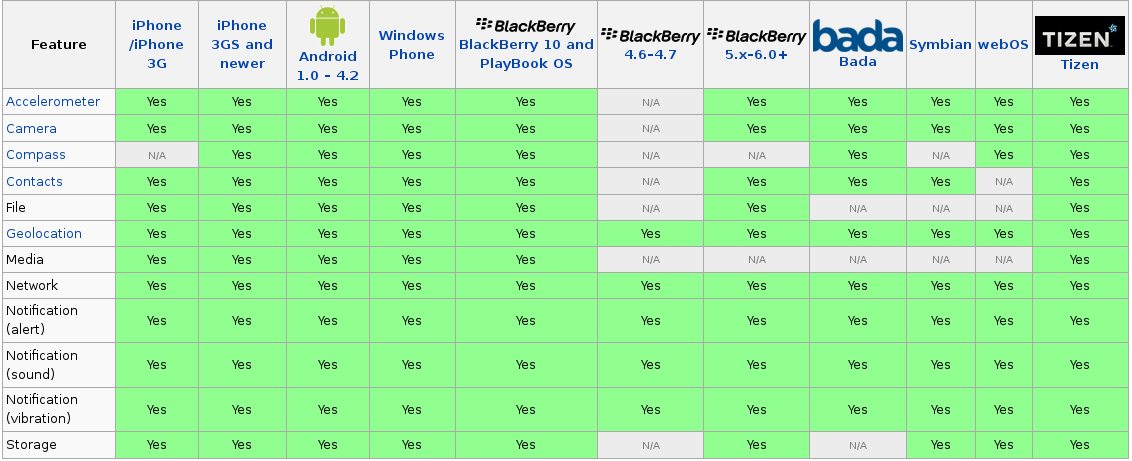
\includegraphics[width=\textwidth]{cordovaFeatures.jpg}
               \caption{Funcionalidades implementadas no projeto Apache Cordova.\label{fig:Cordova}}
    \end{center}
\end{figure}

\end{frame}

\begin{frame}
\frametitle{Metodologia - Processo de software }

Para o  processo de desenvolvimento foi escolhido o OpenUp, justamente por este ser incremental e possuir uma alta gama de artefatos, características aprováveis para o desenvolvimento de algo complexo como um jogo.
\end{frame}

\begin{frame}
\frametitle{Metodologia  - OpenUP}

\begin{figure}[!htbp]
    \begin{center}
        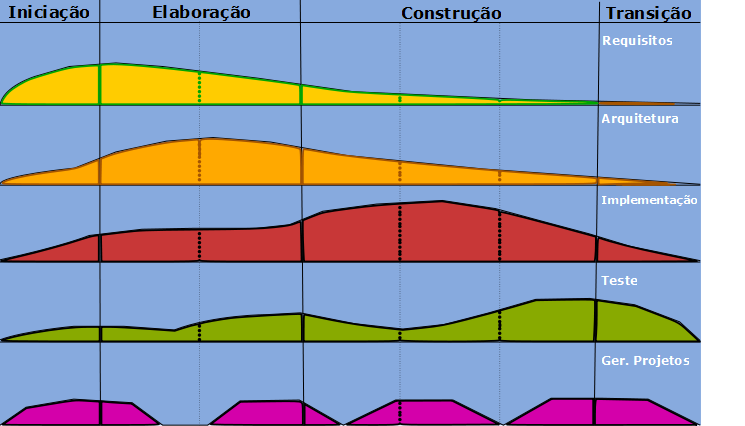
\includegraphics[width=\textwidth]{openupcicle.png}
               \caption{Ciclo de vida do software no OpenUP.\label{fig:OpenUp}}
    \end{center}
\end{figure}

\end{frame}



\begin{frame}
\frametitle{Metodologia  - Fazes macro do desenvolvimento}
  \begin{itemize}
  \item \textbf{Concepção}:  Nesta fase será feita uma análise nos riscos e requisitos do trabalho proposto bem como dar-se-á início ao GDD \textit{Game Document Design} (ou documento de design do jogo);
  \item \textbf{Elaboração}: Esta fase detalhará o funcionamento arquitetural do aplicativo, e de ser concluída a construção do GDD.
  \item \textbf{Contrução}: É neste estágio que a criação do aplicativo acontecerá, em um primeiro momento da forma de um demo, e posteriormente como uma aplicação completa.
  \item \textbf{Transição}: Baterias de testes e a documentação dos resultados será desenvolvido neste estágio.
  \end{itemize}

  \end{frame}

\begin{frame}
\frametitle{Cronograma}

O cronograma foi especificado de acordo com o detalhado na metodologia, suas datas estão especificadas de acordo com dias úteis disponíveis no calendário.\\
\begin{table}[!htbp]
                           \begin{center}
                \begin{tabular}{ | l | l | l | l | l |}
                \hline  
                \textbf{Identificador}& \textbf{Tarefa} &  \textbf{Duração} & \textbf{Início} & \textbf{Término} \\  \hline
                1 & Concepção & 5 dias & 1 agosto & 7 agosto \\  \hline
                2 & Elaboração & 15 dias & 8 agosto & 29 agosto \\  \hline
                3 & Contrução & 15 dias & 30 agosto & 19 setembro \\  \hline
                4 & Contrução & 10 dias & 31 agosto & 3 outubro \\ \hline
                  & Total & 45 dias & 1 agosto & 3 outubro \\
                \hline
                \end{tabular}
            \end{center}
               \caption{Cronograma do projeto. \label{fig:Cordova}}
\end{table}

\end{frame}

\begin{frame}
\frametitle{Dúvidas?}
Dúvidas?
\end{frame}

\begin{frame}
\frametitle{Obrigado.}
Obrigado.
\end{frame}

\end{document}

